\documentclass{article}
\usepackage{tikz}
\begin{document}

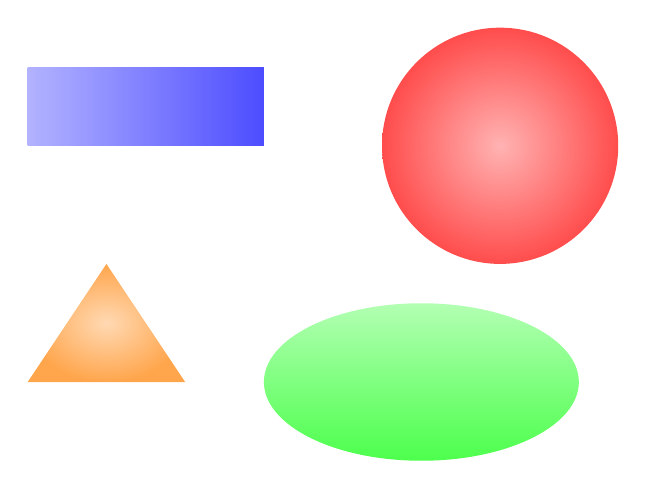
\begin{tikzpicture}[scale=1]

  % --- Shaded rectangle (horizontal gradient) ---
  \shade[left color=blue!30, right color=blue!70]
    (0,0) rectangle (3,1);

  % --- Shaded circle (radial gradient) ---
  \shade[inner color=red!30, outer color=red!70]
    (6,0) circle (1.5);

  % --- Shaded ellipse (vertical gradient) ---
  \shade[top color=green!30, bottom color=green!70]
    (5,-3) ellipse (2 and 1);

  % --- Shaded triangle (custom gradient) ---
  \shade[inner color=orange!30, outer color=orange!70]
    (0,-3) -- (2,-3) -- (1,-1.5) -- cycle;

\end{tikzpicture}

\end{document}
